\section{System Model}\label{sec_system}
The system model is composed of three parts: software applications, an execution platform, and an allocation scheme. In this section, we show models of the different parts and describe them in detail. For smooth reading, first we list the main mathematical notations used throughout the paper, such as to define the system model and the software allocation problem.
 \begin{figure}[!h]
 \centering
 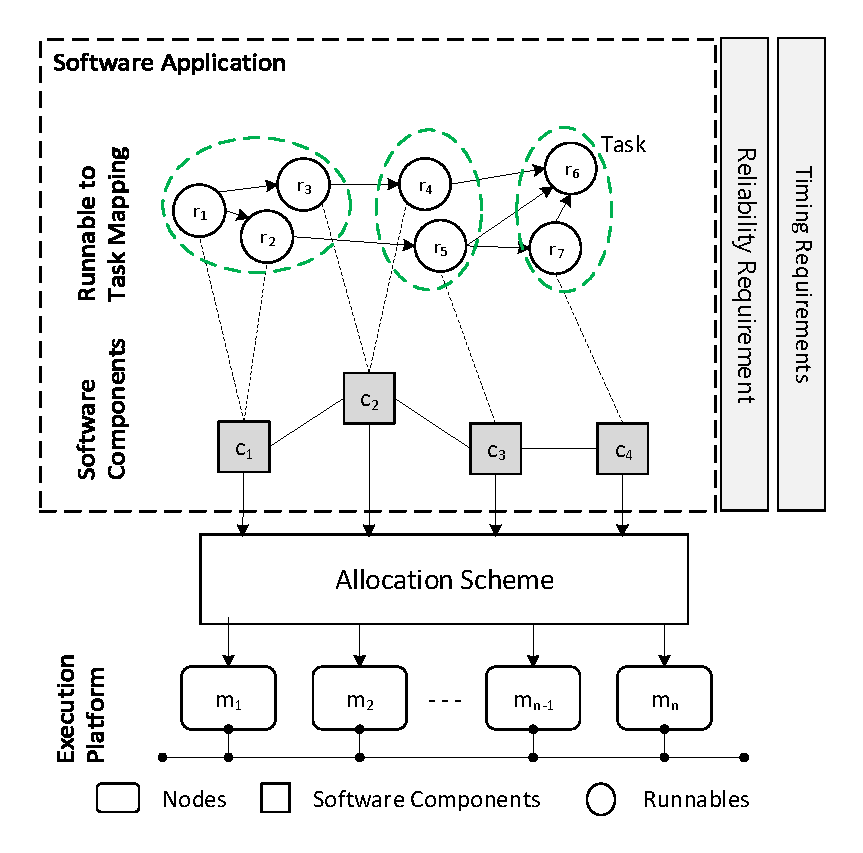
\includegraphics[scale=0.6]{softwareallocation}
 \caption{System Model.}
 \label{fig_softwareallocation}
 \end{figure}
\begin{table}[]
	\small
\begin{tabular}{@{}llp{0.55\textwidth}@{}}
\toprule
 & Notation                        & Description                                             \\ 
\midrule
 &/* Application related */&\\
$\bullet$ & \ttsexp{A}{A}[k]     	            & software applications* \\
$\bullet$ & \sexpsp{C}{c}     		             & software component types of \ttssb{A}[k]**\\
$\bullet$ & \sexpss{Q}{q}    		            & component replicas of type \ttsss{c}\\
$\bullet$ & \sexpss{R}[i]{r}[j]   	             & runnables that implement \ttsss{c}\\
$\bullet$ & \sexpss{H}[i,j]{r}[h]              & runnables that implement $\sss{q}[k][i,j]$\\
$\bullet$ & $\sss{g}[k][r]$   		           & directed acyclic graph of $\bigcup\sss{Q}$ \\
$\bullet$ & $V(g)$   		 & node/vertices of graph $g$\\
$\bullet$ & $E(g)$   		 & links/edges of graph $g$\\
&/* Execution platform related */ &\\
$\bullet$ & \ttsexp{N}{n}         	            & computation (or computing) nodes      \\
$\bullet$ & B         						           & shared CAN bus   \\
$\bullet$ & \ttsexp{M}{m}         	           & messages on the CAN bus   \\
$\bullet$ & \sexpsp{\Gamma}{\Gamma}  & end-to-end chains             \\
$\bullet$ & \ttsss{\Gamma}$=(e_i)_{i=1}^Z$   & a chain of tasks or messages $e$\\ 
$\bullet$ & $\pi_i(\sss{\Gamma})$ & the $i^{th}$ element in \ttsss{\Gamma}\\
$\bullet$ & \multicolumn{2}{p{0.8\textwidth}}{$\tau,c,m,\gamma$ denote iterator variables,  respectively for task, component, chain and node, e.g., $\forall \tau \in  \ssp{T}$.***}\\
 &/* Mapping related */&\\

$\bullet$ & \sexpsp{\textbf{x}}{\textbf{x}}[k]:$\bigcup{\sss{Q}}\mapsto M$            & a mapping vector from \ttssp{Q} to $M$             \\
$\bullet$ & \multicolumn{2}{p{0.8\textwidth}}{$k,i,j$ denote iterator index-variables,  respectively for the mapping vector \ttx, and rows and columns of the matrix \ttxsp{k}, e.g., \ttxkij.***}\\
$\bullet$ & $\sss{g}[k][\tau](\x)$   		           & directed acyclic graph of tasks\\
&/* Functions related */ &\\

$\bullet$ & $Power(\textbf{x})$                		& total power consumption of  $A$ in \ttx    \\
$\bullet$ & $Reliability_{a}(\x)$      					& application reliability  of $a\in A$ in \ttx              \\
$\bullet$ & $ResponseTime_{\tau}(\x)$     		& response time of  $\tau \in V(\sss{g}[k][\tau])(\x)$                       \\
$\bullet$ & $Delay_\gamma(\x)$            			& age delay of $\gamma \in \ssp{\Gamma} $   in \ttx     \\
\bottomrule\\
\end{tabular}
{\footnotesize 
	*Note: the total elements in a set $S$ is denoted by \ttn{S}, e.g., \ttn{A} denotes the number of applications in the set $S$, essentially it refers to its cardinality.\\
	** For readability, we prefer to use \ttsss{S} in place of $\sss{S}[A_k]$. \\
   *** IFor other uses of the iterators, they are defined in the context.}
 
\end{table}

\subsection{Software Applications}
The software applications are user-defined software systems, e.g., x-by-wire, electronic throttle control, flight control, etc., that are developed using software components \cite{softwarecomponents}\cite{Crnkovic2002BuildingSystems}. A software application $A_k$ is associated with high-level and user defined requirements $(\bigcup_i e2ereq_i,relreq,cl):\mathbb{R}^+\times [0,1]\times \mathbb{I}^+$, where the tuple elements denote, respectively the reliabiliy requirement, end-to-end timing requirements and criticality-level of the application $A_k$, and we access the elements through the projection symbol $\pi$ as $\pi_{e2ereq_i}(A_k)$, e.g., $\pi_{e2ereq_1}(A_2)$ means the first end-to-end requirement of application $A_2$. The critical level signifies the importance of an application over other applications that have lower criticality levels, thus prioritizing the application during resource contention. The criticality levels are defined systematically, e.g., following the hazard analysis according to ISO 26262 standard. The end-to-end timing requirements define the timing constraints over end-to-end functional behaviors of applications, which are referred to as \textit{cause-effect chains}, and finally the reliability requirement defines the expected reliability goal of an application which is discussed further in Subsection \ref{subsec_reliability_constraint}. 

The software applications are run in parallel and therefore can potentially be distributed on different computation nodes \ttsexp{M}{m}, and we assume the nodes are heterogeneous with respect to processor speed, failure-rate and power consumption as indicated by the tuple $(hz, \lambda, p)$, respectively. 

%$\bigcup_{i=1}^{N_a} A_i$ 
\begin{definition}[Software Application Model]
It is modeled as a set of communicating software components which is associated to a function behavior that is modeled as \textit{directed acyclic vertex-weighted} graph $\langle V_\tau,L_\tau, w\rangle$ of periodic task nodes $V_\tau$, where $a_{ij}\in L_\tau$ refers to the data-flow link from node $\tau_i$ to node $\tau_i$ and $i \neq j$. The computation cost $w(\tau)=\langle \bigcup e_{m_i},D,P, m\rangle$ refers, respectively the worst-case execution times {WCET} on nodes $M$, deadline and period, and its mapping to a node $m\in M$.
\end{definition}%  \textit{undirected} graph $\langle V_c,L_c\rangle$ of software component nodes, where $a_{ij}\in L_c$ refers to the communication link from node $c_i$ to node $c_j$. It is

Multiple applications can be executed on the same computation node(s) and can share the CAN bus. Since the applications can have different criticality requirements, the execution platforms should provide a separation mechanism in order to avoid interference of lower-critical applications on higher-critical applications, e.g., faults propagation, also known as   \textit{mixed-critical} design \cite{Vestal2007PreemptiveAssurance}, which is an existing practice in avionics and also trending in other domains, e.g., automotive, where  safety-critical applications, such as x-by-wire and electronic throttle control systems, are required to be consolidated with the infotainment system on the same ECUs \cite{bibid}.

\subsection{Scheduling Software Applications}
The applications are scheduled on the heterogenous execution platform by considering their respective requirements such as the criticality levels, reliability requirements, and end-to-end timing requirements. There are several techniques in the literature that deal with the scheduling of mixed-critical applications on a \textit{uniprocessor} systems \cite{Vestal2007PreemptiveAssurance}. In our problem, though distributed applications, each task is mapped to a single node, and the mapping is static. In this case, the schedulability is of tasks can be performed per node, that is using the approach applied to uniprocessing nodes. Therefore, we say the distributed applications are schedulable if the tasks, messageges, and cause-effect chains in the system meet their respective deadlines in the midst of power consumption and reliability constraints. 

In this work, we consider the \textit{partitioned criticality (PA)}  technique to schedule the mixed-crtitica applications, which basically prioritizes higher critical applications over their lower critical counterparts. In contrast to other techniques, PA does not require a runtime monitoring of tasks, e.g., using servers \cite{AbeniIntegratingSystems,Ashjaei2017DesigningSystems,Inam2014ThePlatforms}, though less efficient. Note: other scheduling techniques can be used on behalf of PA with our approach.

\subsubsection{Scheduling Tasks and Messages}\label{subsec_responsetimeanalysis}
We assume tasks are scheduled using the \textit{fixed-priority preemptive scheduling polity} (FPPS). Initally, applications are priortized based on their criticality levels followng the PA technique, and within each application the tasks are prioritized with the \textit{deadline monotonic} (DM) priorities assignment. 

\[cri(A_h)>cri(A_l)\implies \forall \tau_1\in\bigcup\sss{T}[h]\tau_2\in\bigcup\sss{T}[l]\ Pri(\tau_1)>Pri(\tau_2)\],
where $cri, pri$ are predicates which detemine the critiality and priority of tasks $\tau_1,\tau_2$, respectively; $\bigcup\sss{T}[h], \bigcup\sss{T}[h]$ are the set of tasks which implement the applications $A_i,A_j$, respectively.

The schedulability of tasks assigned to a node is performed uisng the classical response-time analysis shown in Equaiton (\ref{eqn_responsetimeanalysis}) \cite{Baruah2011Response-timeSystems,Baruah2011Response-timeSystems}, which computes the worst-case response time of each task $R_\tau$. According to the analysis, if the response time of each task is less than or equal to its deadline, that is $R_\tau\leq Deadline_\tau$, the taskset is schudlable otherwise it is not. 

\begin{align}
\label{eqn_responsetimeanalysis}
R_\tau=c_\tau+\sum_{\gamma \in H\!P(\tau)}{\ceil[\Big]{\frac{R_\tau}{P_{\tau_{hi})}}*c_\gamma}},
\end{align}
 where $\gamma\in H\!P(\tau)$ is element of the higher-priority tasks returned by $H\!P$.

In this work, we assume heterogenous computation nodes, therefore the schedule that delivers lower power-consumption of a node is considered the effective and efficient. The power-consumption of a node is computed linearly from the utilization of a taskset mapped to a specific node as well as from its power-specification parameters, and is discussed in detail in Subsection \ref{sec_problem}.

Unlike the tasks, the messages in the CAN bus $B$ are scheduled using a non-preemptive and fixed schduling policy. Similar to the mixed-criticality of tasks, the messages in the can should be separated as well for different critial applications, which is achieved by applying the PA technique. In this case though, the priorities of messages are inherited from the send tasks, $pri(m)=pri(\tau)|\tau = pre(m)$, where $pre(\tau)$ is a predicate that computes the predecessor of task $\tau$ from the tasks graph $g_\tau$. The schdulability of messages is checked using the classical response-time analysis of messages in CAN network, as shown in Equation ().
\begin{align}
\label{eqn_responsetimeanalysisCAN}
R_\tau=c_\tau+\sum_{\gamma \in H\!P(\tau)}{\ceil[\Big]{\frac{R_\tau}{P_{\tau_{hi})}}*c_\gamma}},
\end{align}


\subsubsection{Scheduling Cause-effect Chains}\label{subsec_causeeffectchains}
The software application can be considered as a set of \textit{cause-effect chains} \sexpsp{\Gamma}{\Gamma}, which are  directed paths in the graph, annotated by end-to-end timing requirements \ttsss{End2end}. They represent sequences of actions triggered usually by external events (or causal actions or stimuli) and produce corresponding effects (or responses), e.g.,  pressing a rotary-wheel to activate a cruise control system, pressing a brake pedal to slow down a car, etc. The end-to-end requirements put upper-bounds on the duration of the stimuli-reponse elapse time. An example of a cause-effect chain is shown in Figure \ref{fig_causeeffectchainntk}, which consists of three independently clocked tasks $\tau_1,\tau_2,\tau_3$, and message $m_1,m_2$. It uses single-register buffers for communication, which is a common practice in control systems design, e.g., automotive software applications.
\begin{figure}
	\centering
	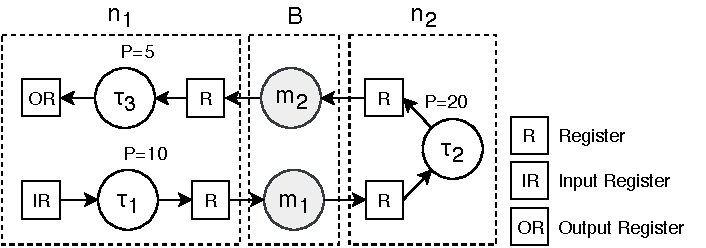
\includegraphics[width=0.7\linewidth]{img/cause_effect_chain_ntk}
	\caption{A Cause-effect Chain, mapped on nodes $n_1$ and $n_2$.}
	\label{fig_causeeffectchainntk}
\end{figure}

The delay of a chain is the duration between the reading of data from the input register by the source task $Source(\sss{\Gamma})$ to the writing of same data to the ouput register by the last (or sink) task $Sink(\sss{\Gamma})$. Since we assume the chains consist of independently clocked tasks, the delay usually varies due the undersampling/and oversampling effects caused as a result. In this work, we are interested on particular types of delays that are widely used in automotive and similar systems such as \textit{age delay} and\textit{ reaction delay}. 
\begin{figure}
	\centering
	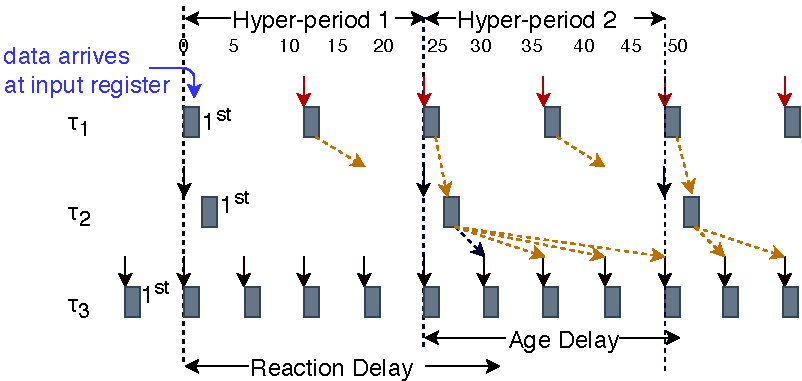
\includegraphics[width=0.9\linewidth]{img/timedchain_ntk}
	\caption{Reaction and Age Delays of the Cause-effect Chain, Shown in Figure {\ref{fig_causeeffectchainntk}}.}
	\label{fig_timedchainntk}
\end{figure}

The difference between the two types of delays is demonstrated in Figure~\ref{fig_timedpath}. The tasks $\tau_1$ and $\tau_2$ execute on node $n_1$, whereas task $\tau_3$ executes on node $n_2$. Note: $\tau_1$ communicates with $\tau_2$ via a CAN bus, which is not shown in the figure for simplicity. The red inverted arrows in the figure represent the reading of data from the input register, whereas the dashed-curve arrows represent the timed paths through which the data propagates from the input to the output of the chain. Thus, the age delay is the time elapsed between a stimulus and its corresponding latest non-overwritten response, i.e., between the $3^{nd}$ instance of  $\tau_1$  and the $10^{th}$ instance of $\tau_3$. It is frequently used in the control systems applications where freshness of data is paramount, e.g., braking a car over a bounded time. And, the reaction delay is the earliest time the system takes to respond to a stimulus that ``just missed" the read access at the input of the chain. Assume that data arrives just after the start of the $1^{st}$ instance of $\tau_1$ execution. The data corresponding to this event is not read by the current instance of $\tau_1$. In fact, the data will be read by the $2^{nd}$ instance of $\tau_1$. The earliest effect of this data at the output of the chain will appear at the $7^{th}$ instance of $\tau_3$, which represents the reaction delay. This delay is useful in body-electronics domain where first reaction to events is important, e.g., in the button-to-reaction applications. For detailed discussion of the different delay semantics, we direct the reader to check research work by Saad et al.~\cite{mubeen2013support}. The age delay is analytically calculated using Equation \ref{eqn_agedelay}, and is explained as follows.
\begin{align}
	\label{eqn_agedelay}
	AgeDelay(\Gamma)=
	\begin{cases}
	\alpha(Sink(\Gamma)-\alpha(Source(\Gamma) + \delta(Sink(\Gamma))& \shortintertext{ (if chain mapped on a single node)}\\
	\sum_{a\in Part(\Gamma)}{AgeDelay(\Gamma)} + \sum_{m\in M'}{\delta(m)}&\shortintertext{ (if chain mapped on multiple nodes)}
	\end{cases}
\end{align}

Assume $\Gamma \in \sss{\Gamma}$ is a chain, if the chain is mapped on a single node, the age delay is a mere difference between the activation of the sink task $\alpha(Sink(\Gamma))$ and the activation of the source task $\alpha(Source(\Gamma))$ plus the worst-case execution time of the sink task. Otherwise, if the chain is mapped on multiple nodes, the delay is compositionally computed as follows: the chain is partitioned  into a set of chains per node, indicated by the predicate $Part(\Gamma)$ and for each partitioned chain $a\in Part(\Gamma)$, the age delay is computed recursively, and the result is added to the response-times of the messages involved in the chain $M'$.

\subsection{AUTOSAR System}\label{subsec_autosarsystem}
The AUTOSAR standard introduced the notion of \textit{Runnables} to facilitate early analysis, that is at the VBF level, and to support interoperability of automotive applications across different execution platforms. Basically, runnables are schedulable pieces of codes similar to tasks. In this work, we assume periodically activated runnables with support for multiple worst-case executions that correspond to the different computation processor types. Unlike tasks, runnables' functional and extra-functional properties, e.g., timing, memory requirements, are part of the AUTOSAR software component specifications. Therefore, the software application model is extended to accommodate the notion of runnables, using the following simplified formal definition.

\begin{definition}[AUTOSAR Software Application Model]
It is modeled as directed acyclic vertex-weighted graph $g_r=\langle V_r, L_r, w, v\rangle$ of runnable nodes $V_r$, where $a_{ij}\in L_r$ represents either a triggering or data-flow link from the runnable $r_i$ to runnable $r_j$ and $i\neq j$. The cost at the node refers to the timing model of the runnable, where the tuple elements, respectively denote execution time on node $m$, deadline and period. Example: Figure \ref{fig_appexample}(a).
\end{definition}

\begin{figure}[h!]
	\centering
	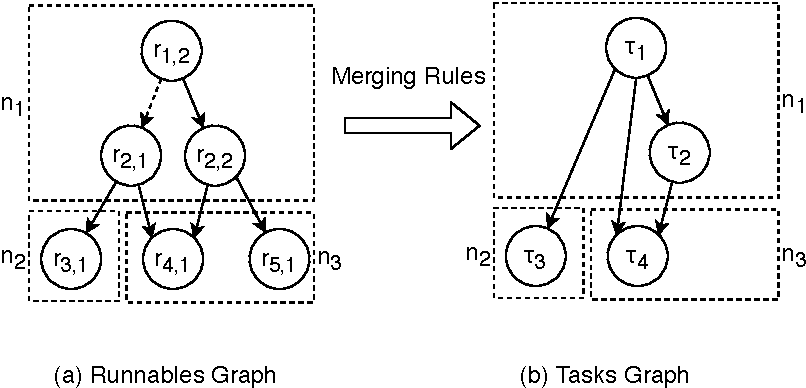
\includegraphics[width=0.7\linewidth]{img/runnable_task_dag}
	\caption[Example of a Software Application.]{Example of a Software Application, Modeled as Directed Acyclic Graph, where $\dashrightarrow$, $\dashrightarrow$ denote triggering link, data-flow link, respectively.}
	\label{fig_appexample}
\end{figure}

\begin{table}
	\parbox{.45\linewidth}{
		\centering
\begin{tabular}{|c|c|c|c|}
	\hline 
	\ttsss{r}[k][i,j] &$m_h$& $(e_h, P)$ & $\prec$ \ttsss{r} [k][i,j]\\ 
	\hline 
	1,1 & 1&$(1,10)$ & 2,1 \\ 
	\hline 
	2,1 &1& $(1,5)$ &  \\ 
	\hline 
	2,2 &1& $(1,15)$ &  \\ 
	\hline 
	3,1 & 2&$(1,20)$ &  \\ 
	\hline 
	4,1 & 3&$(1,10)$ &  \\ 
	\hline 
	5,1 & 3&$(1,20)$ &  \\ 
	\hline 
\end{tabular} 
		\caption{Runnables Timing Specifications.}
	}
	\hfill
	\parbox{.45\linewidth}{
		\centering
		\begin{tabular}{|c|c|c|}
			\hline 
			\ttsss{\tau} &$\bigcup\sss{r}[k][i,j]$& $(e_h,P)$ \\ 
			\hline 
			1 & 1,2;2,1 &  $(2,5)$\\ 
			\hline 
			2& 2,2 &  $(1,15)$\\ 
			\hline 
			3& 3,1 &  $(1,20)$\\ 
			\hline 
			4 & 4,1;5,1 &  $(1,10)$\\ 
			\hline 
		\end{tabular} 
		\caption{Tasks-Runnables Mappings.}
	}
\end{table}

According to AUTOSAR specification \cite{AUTOSAR2017SpecificationSoftware}, runnables are mapped to tasks, and the tasks execute the runnables respecting their timing specifications. In the mapping process, one or more runnables can be merged to optimize the runtime execution by reducing the number of schedulable tasks. Thereore, through the mappings, eventually runnables graphs are refined by tasks graphs as shown in Figure{\ref{fig_appexample} (b). In this work, the following rules are applied in order to merge any runnables $a,b$, that is the link $(a, b)\in L_r$ merges to a task node $v\in V(g_\tau)$, if the following rules satisfy':
\begin{enumerate*}[label=(\roman*)]
\item the runnables are co-hosted in the same computation node, i.e., $a\mapsto m \land b\mapsto m$
\item activation periods of the runnables are the same, i.e., $a.P = b.P$
\end{enumerate*}

If the rules are satisfied, the task's timing specifications are set as follows: i) the WCET of the task is set to the sum of the WCET of the runnables, $v.e_i=a.e_i + b.e_i$, ii) the period and deadline of the task is  set to the least-common multiple (LCM) of the runnables' periods, $v.P=v.D=LCM(a.P, b.P)$. Otherwise, runnables are not merged, instead, each runnable that is not merged is mapped to a task while preserving the timing specifications of runnables on the tasks.

% Following the grouping of runnables to tasks, We assume runnables communicate (or send data messages) at the end of the corresponding tasks' executions. The messages are packed into a single frame if destined to the same node otherwise each runnable communicats across a shared bus via a dedicated message entity, which is schedulable by the CAN bus controller. In essence, the assumed read-exec-write semantics of the runnables lowers the number of schedulable messages entities in the bus by facilitating packing of signals at the expense of restrictive (or less flexible) inter-runnables communication.

% Furthermore, we assume fixed and dynamic preemptive scheduling policies, that is each tasks sets allocated to a node must be schedulable according to the choice of the scheduling policy. For convenience, we assume priorities are assigned to tasks according to Rate Monotonic (RM) for the case of fixed scheduling policy, that is a task with a lower period get a higher priority.

\subsection{Execution Platform}
The execution platform provides computation and communication resources to the user applications, and is modeled as a \textit{complete} graph $\langle M,L^m\rangle$ of computation nodes, where $(m_i,m_j)\in L^m \land i\neq j$ refer to the communication links of the nodes, which are realized by a network bus, e.g., CAN. The computation nodes are heterogeneous with respect to parameters defined as a tuple $\langle hz, \lambda, p \rangle$, respectively denote processor speed, failure-rate and power consumption specifications. The allocation scheme is a mapping table $f:C\mapsto M$ from software components to computation nodes, where $C=\bigcup_{i=1}^{|A|} {V(A_i)}$ is the \textit{infinitary} union of the user applications' vertices, which denote nodes o software components.

\subsection{Fault-tolerant Software Application Model}
Redundancy is the most common way to increase the reliability of an application. It can be implemented according to different schemes, such as hot stand-by, cold stand-by, etc~\cite{Dubrova2013Fault-tolerantDesign}. In this work the details of the redundancy scheme are abstracted away under the following assumptions: i) Hot stand-by redundancy technique is used for the replacement of failed components, which are identical and are allocated on different nodes, ii) software components need to be replicated if the application's reliability requirement is not met without replication, otherwise they are not replicated, iii) the time needed to detect and replace a faulty component is considered negligible and will not be taken into account in the response time analysis of tasks and delay calculation of cause-effect chains, iv) Because of its simplicity, the mechanism for detection and replacement of faulty components will be considered fault-free, and therefore will not be included in the reliability calculations.

We denote the $k^{th}$ replica of a software component $c$ as $c^k$, with $1\le k\leq K$; where $K$ is the maximum number of replicas allowed for each application component.

%\subsection{Platform Model}
%The application is deployed on a network of heterogeneous computing nodes that are connected via a reliable communication network, the CAN bus. The computation node is specified as a 3-tuple $\langle hz, \lambda, p \rangle$, respectively, refer to the processor frequency, failure-rate and power consumption of a computation node. Due to the heterogeneity assumption of the processors, an application maybe be deployed on nodes with higher processor frequencies, and therefore fewer number of nodes in order to minimize the total power consumption of the system. However, due to the application reliability requirement, the application could be deployed differently, and with more resources. The CAN bus is considered reliable, for instance through redundancy. Therefore, its exclusion from the overall calculation of the system's reliability does not impact our proposed software allocation. %Figure~\ref{fig_softwareallocation} illustrates an overview of an AUTOSAR software application deployment on a set of computational nodes via a software allocation scheme that is discussed in Section~\ref{sec_allocation}.




%\subsection{AUTOSAR Software Application Model}
%AUTOSAR software applications are constructed from communicating AUTOSAR application components $\bigcup_{i=1}^{I} C_i$, where the component $c_i^k$ is the $k^{th}$ replica of the component type $C_i$ and $I$ is the number of software component types (or the cardinality of the infinitary union). Each software component co-hosts a set of runnables $R^*\subseteq R$ that are disjoint.
